\documentclass[
  captions=tableheading,
  bibliography=totoc, 
  titepage=firstiscover,
]{scrartcl}

\usepackage{blindtext} %neuer input

\usepackage{longtable} % Tabellen über mehrere Seiten

\usepackage[utf8]{inputenc} %neuer input

\usepackage{scrhack}

\usepackage[aux]{rerunfilecheck} %Warnung falls nochmal kompiliert werden muss

\usepackage{fontspec} %Fonteinstellungen

\recalctypearea{}

\usepackage[main=ngerman]{babel} %deutsche Spracheinstellung

\usepackage{ragged2e} %neuer input

\usepackage{amsmath, nccmath}

\usepackage{amssymb} %viele mathe Symbole

\usepackage{mathtools} %Erweiterungen für amsmath


\DeclarePairedDelimiter{\abs}{\lvert}{\rvert}
\DeclarePairedDelimiter{\norm}{\lVert}{\rVert}

\DeclarePairedDelimiter{\bra}{\langle}{\rvert}
\DeclarePairedDelimiter{\ket}{\lvert}{\rangle}

\DeclarePairedDelimiterX{\braket}[2]{\langle}{\rangle}{
#1 \delimsize| #2
}

\NewDocumentCommand \dif {m}
{
\mathinner{\symup{d} #1}
}


\usepackage[
  math-style=ISO,
  bold-style=ISO,
  sans-style=italic,
  nabla=upright,
  partial=upright,
  warnings-off={
    mathtools-colon,
    mathtools-overbracket,
  },
]{unicode-math}

\setmathfont{Latin Modern Math}
\setmathfont{XITS Math}[range={scr, bfscr}]
\setmathfont{XITS Math}[range={cal, bfcal}, StylisticSet=1]


\usepackage[
  locale=DE,
  separate-uncertainty=true,
  per-mode=reciprocal,
  output-decimal-marker={,},
]{siunitx}

\usepackage[autostyle]{csquotes} %richtige Anführungszeichen

\usepackage{xfrac}

\usepackage{float}

\floatplacement{figure}{htbp}

\floatplacement{table}{htbp}

\usepackage[ %floats innerhalb einer section halten
  section,   %floats innerhalb er section halten
  below,     %unterhalb der Section aber auf der selben Seite ist ok
]{placeins}

\usepackage[
  labelfont=bf,
  font=small,
  width=0.9\textwidth,
]{caption}

\usepackage{subcaption} %subfigure, subtable, subref

\usepackage{graphicx}

\usepackage{grffile}

\usepackage{booktabs}

\usepackage{microtype} %Verbesserungen am Schriftbild

\usepackage[
backend=biber,
]{biblatex}

\addbibresource{../lit.bib}

\usepackage[ %Hyperlinks im Dokument
  german,
  unicode,
  pdfusetitle,
  pdfcreator={},
  pdfproducer={},
]{hyperref}

\usepackage{bookmark}

\usepackage[shortcuts]{extdash}

%\usepackage{warpcol}


\begin{document}
    \title{V702 Aktivierung mit Neutronen }
    \author{  
    Tobias Rücker\\
    \texorpdfstring{\href{mailto:tobias.ruecker@tu-dortmund.de}{tobias.ruecker@tu-dortmund.de}
    \and}{,} 
    Paul Störbrock\\
    \texorpdfstring{\href{mailto:paul.stoerbrock@tu-dortmund.de}{paul.stoerbrock@tu-dortmund.de}}{}
    }
    \date{Durchführung: 26.05.2020, Abgabe: 02.06.20 \vspace{-4ex}}
\maketitle
\thispagestyle{empty}

\newpage
\tableofcontents
\thispagestyle{empty}
\newpage

% Ziel %%%%%%%%%%%%%%%%%%%%%%%%%%%%%%%%%%%%%%%%%%%%%%%%%%%%%%%%%%%%%%%%%%%%%%%%%%%%%%%%%%%%%%%%%%%%%%%%%%%%%%%%%%%%%%%%%%%%%%%%%%%%%%%%%%%%%%%%%%%%%%%%%%%%%%%%%%%%%%%%%%%%%%%%%%%%%%%%%%%%%%%%%%%%%%%%%%%%%%%%%%%%%%%%%

\setcounter{page}{1}
\section{Ziel}\justifying
Die Kenntnis über die Stabilität von Atomen und den Verlaufsprozess von verschiedenen
Zerfällen spielt nicht nur bei Messungen in der Physik, sondern vor allem auch in der 
Medizin, zum Beispiel in der Krebsbehandlung, eine Rolle. Daher wird im Folgenden die Halbwertszeit von
zwei Materialien bestimmt, indem diese mit energiearmen Neutronen beschossen werden und die Teilchen mittels 
einem Geiger-Müller-Zählrohr gezählt werden.

% Theorie %%%%%%%%%%%%%%%%%%%%%%%%%%%%%%%%%%%%%%%%%%%%%%%%%%%%%%%%%%%%%%%%%%%%%%%%%%%%%%%%%%%%%%%%%%%%%%%%%%%%%%%%%%%%%%%%%%%%%%%%%%%%%%%%%%%%%%%%%%%%%%%%%%%%%%%%%%%%%%%%%%%%%%%%%%%%%%%%%%%%%%%%%%%%%%%%%%

\section{Theorie}\justifying
Die Stabilität von Atomen hängt stark von dem Verhältnis der Protonen und Neutronen ab. Sind
Atome nicht stabil, zerfallen sie zu stabilen oder instabilen Kernen, wo bei instabilen der Zerfallsprozess
noch nicht beendet ist.  Eine wichtige Eigenschaft des Zerfallsprozesses stellt die Halbwertszeit T
dar. Sie beschreibt die Zeit, nach der die Hälfte der Kerne einer Menge zerfallen sind.
Für die Messung der Halbwertszeit in einer Größenordnung von Stunden und Sekunden werden
stabile Kerne mit Neutronen beschossen. Diese Kerne werden nach der Absorption des Neutrons zu einem Zwischenkern $A^*$, welcher
auch Compoundkern genannt wird. Die Energie des Neutrons verteilt sich auf die anderen Nukleonen,
wodurch diese in höhere Energiezustände gebracht werden. Bei Neutronen mit geringen 
Energien kann kein Nukleon abgestoßen werden, weshalb es unter Aussendung eines Gammaquants in den Grundzustand übergeht \cite{V702}
\begin{align}
    \ce{_z^mA + _0^1n -> _z^{m+1}A^* -> _z^{m+1} A + \symup{\gamma}}. \label{eq:1} %hier steht das erste plus im exponenten
\end{align}
Dabei gibt m die Massenzahl, z die Ordnungszahl, n das eingesendete Neutron, A den beschossenen Kern,
$A^*$ den Zwischenkern und $\gamma$ den ausgesendeten Gammaquant an. Durch das zusätzliche
Neutron ist der Kern nun instabil und zerfällt \cite{V702}
\begin{align}
    \ce{_z^{m+1}A -> _{z+1}^{m+1}C + \symup{\beta}^- + E_{\text{kin}} + \bar{\symup{\nu}}_e } \label{eq:2}.
\end{align}
Hierbei ist C der aus dem Zerfall entstehende Kern, $\beta ^-$ ein Elektron und $\bar{\nu}_e$ ein Elektron-Antineutrino.
Die Masse der Teilchen auf der linken Seite der Reaktionsgleichung ist größer als die der Teilchen auf
der rechten Seite. Diese Energie geht in Form von kinetischer Energie an das Elektron und
Elektron-Antineutrino. Um möglichst viele Zerfälle für eine Messung zu erzeugen wird ein
entsprechend hoher Wirkungsquerschnitt $\sigma$ benötigt. Der Wirkungsquerschnitt beschreibt
die Fläche, die der Atomkern haben müsste, damit jedes Neutron mit der Fläche wechselwirkt.
Für eine geringe Energie der Neutronen gegenüber des Zwischenkerns ergibt sich folgende
Proportionalität für den Wirkungsquerschnitt \cite{V702}
\begin{align}
    \sigma \sim \frac{1}{v}, \label{eq:3}
\end{align}
wobei v die Geschwindigkeit der Neutronen ist.
Aufgrund der Proporionalität sind niederenergetische Neutronen für die Messung notwendig,
was verständlich ist, da eine kleinere Energie eine geringere Geschwindigkeit bedeutet
und sich das Neutron dadurch länger in der Einwirkssphähre befindet.\\
Für die Erzeugung von Neutronen kann die Reaktion von Beryllium mit 
Alpha-Teilchen genutzt werden \cite{V702}
\begin{align}
    \ce{ ^9 Be + _2^4 \symup{\alpha} -> _6^{12} C + _0^1n }. \label{eq:4}
\end{align}
Die $\alpha$-Teilchen entstehen dabei aus dem Zerfall von $^{226} $Ra-Kerne.
Da die Neutronen nach der Reaktion noch zu energiereich sind, wird eine dicke Materieschicht eingebracht,
durch die die Neutronen hindurchdiffundieren müssen. Die Kerne davon sollten auf
einer gleichen Größenordnung wie die Neutronen sein, damit der Energieübertrag am größten ist.
Daher eignet sich Paraffin dafür. Ein schematischer Aufbau für so eine Quelle ist in der folgenden Abbildung
dargestellt:
\begin{figure}[H]
    \centering
    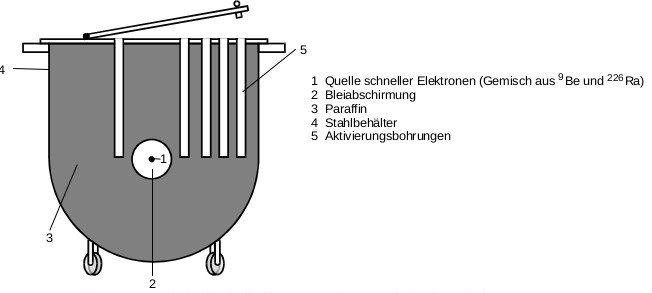
\includegraphics[width=\linewidth]{images/neutron_quelle.jpg}
    \caption{Schematischer Aufbau einer Neutronenquelle \cite{V702}.
    Durch den Zerfall von Radium-Kernen entstehen $\alpha$-Teilchen,
    welche mit den Beryllium-Atomen wechselwirken. Dadurch entstehen Neutronen,
    welche im Paraffin einen Teil ihrer Energie abgeben und damit abgebremst werden.
    }
    \label{fig:1}
\end{figure}
\flushleft{Die\,}\justifying abgebremsten Neutronen haben eine kinetische Energie, welche der mittleren Energie der Umgebung entspricht und
werden thermische Neutronen genannt.\\
Für Messungen wird eine zylindrische Probe in einen Aktivierungsschacht gebracht.
Da es schwer ist die Zerfallsrate pro Zeit genau zu bestimmen, wird die Anzahl der 
Zerfälle über ein Zeitintervall $\Delta t$ betrachtet. Dafür ergibt sich ein
einfacher exponentieller Zusammenhang \cite{V702}
\begin{align}
    N_{\Delta t} (t) = N_0 (1-e^{\lambda \Delta t}) e^{- \lambda t}. \label{eq:5} 
\end{align}
Dabei stellt $N_0$ die zu Messbeginn vorhandene Anzahl an instabilen Kernen und $\lambda$ die Zerfallskonstante dar.
Die Halbwertszeit lässt sich über die Formel \cite{V702}
\begin{align}
    T=\frac{\ln(2)}{\lambda} \label{eq:6}
\end{align}
berechnen.\\
Eine geeignete Wahl des Zeitintervalls ist wichtig, da es ansonsten zu hohen
statistischen oder systematischen Fehlern kommt.\\
Manche Materialien wie Rhodium haben zwei Zerfallsketten\\
\begin{align}
\ce{^{103}_{45}Rh + n}  
\begin{cases}
    \ce{\stackrel{10\%}{\to} ^{104i}_{45}Rh +\symup{\gamma} -> ^{104}_{46}Pd +\symup{\beta}^- + \bar{\symup{\nu}}_e }\\
    \ce{\stackrel{90\%}{\to} ^{104}_{45}Rh ->  ^{104}_{46}Pd +\symup{\beta}^- + \bar{\symup{\nu}}_e }
\end{cases}.\text{\cite{V702}} \label{eq:7}
\end{align}
Das i beim Rhodium steht für einen isomeren Kern, welcher sich nur in der Energie und
Halbwertszeit vom Rhodium-Kern unterscheidet.\\
Da der nicht-isomere Kern kurzlebiger ist, wird ab einem gewissen Zeitpunkt $t^*$ hauptsächlich
der isomere Kern gemessen, was in der folgenden Abbildung zu erkennen ist:
\begin{figure}[H]
    \centering
    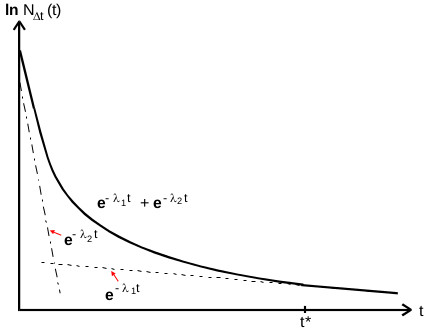
\includegraphics[width=\linewidth]{images/Rh_theo.jpg}
    \caption{Logarithmische Darstellung eines zeitlichen Zerfalls mit
    2 Zerfallsketten \cite{V702}.
    Die gestrichelten Linien zeigen den potentiellen Verlauf der Geraden für die 
    einzelnen Komponenten der Zerfallsreaktion. Der Zeitpunkt $t^*$ markiert den Übergang, ab
    dem der kurzlebigere Kern kaum noch einen Einfluss hat und eine Gerade entsteht.
    }
    \label{fig:2}
\end{figure}


% Versuchsaufbau + Versuchsdurchführung %%%%%%%%%%%%%%%%%%%%%%%%%%%%%%%%%%%%%%%%%%%%%%%%%%%%%%%%%%%%%%%%%%%%%%%%%%%%%%%%%%%%%%%%%%%%%%%%%%%%%%%%%%%%%%%%%%%%%%%%%%%%%%%%%%%%%%%%%%%%%%%%%%%%%%%%%%%%%%%%%%%%%%%%%%%%%%%%%%%%%%%%%%%%%%%%%%

\section{Versuchsaufbau und Versuchsdurchführung}\justifying

    \flushleft{Um\:}\justifying die Halbwertszeit der gewählten Materialien bestimmen zu können, wird der folgende Aufbau verwendet.
    \begin{figure}
        \centering
        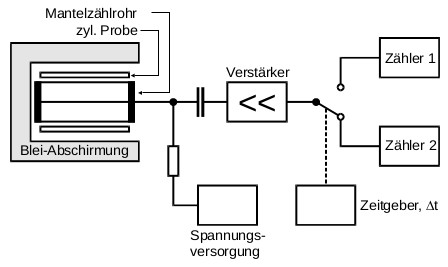
\includegraphics[width=\textwidth]{images/aufbau.jpg}
        \caption{Schematischer Aufbau der Messaparatur \cite{V702}. Innerhalb der Bleiabschirmung befindet sich
        die zylindrische Probe, welche untersucht werden soll. Die elektrischen Signale,
        welch durch die Zerfälle entstehen werden an einen Verstärker weitergeleitet und
        anschließend vom Zählrohr gemessen. Dabei wird nach dem Zeitintervall $\Delta t$ periosdisch auf
        den jeweils anderen Zähler umgeschaltet.
        }
        \label{fig:3}
    \end{figure}
    \flushleft{Zuerst\:}\justifying wird die Untergrundrate $U_N$ bestimmt, dafür wird keine Probe auf das Geiger-Müller-Zählrohr gesteckt.
    Um den Fehler möglichst gering zu halten, wird eine  minimale Messzeit von 500 bis $\SI{600}{\second} $ gewählt. Das Zeitintervall
    wird dabei an dem Codierschalter an der Frontplatte eingestellt.

    
    \flushleft{Für\:}\justifying die Messung der Proben werden diese auf das Geiger-Müller-Zählrohr gesteckt und ein,
    für die Messung geeignetes, Zeitintervall eingestellt. Dieses kann von Probe zu Probe variieren und muss
    eventuell durch Vormessungen bestimmt werden.

% Auswertung %%%%%%%%%%%%%%%%%%%%%%%%%%%%%%%%%%%%%%%%%%%%%%%%%%%%%%%%%%%%%%%%%%%%%%%%%%%%%%%%%%%%%%%%%%%%%%%%%%%%%%%%%%%%%%%%%%%%%%%%%%%%%%%%%%%%%%%%%%%%%%%%%%%%%%%%%%%%%%%%%%%%%%%%%%%%%%%%%%%%%%%%%%%%%%%%%%

\section{Auswertung}
Für die Erstellung der Graphen wird matplotlib \cite{matplotlib} verwendet.
Alle in der Auswertung befindlichen Messungenauigkkeiten, welche sich durch die gauß'sche Fehlerfortpflanzung ergeben,
werden wiederum mit Uncertainties \cite{uncertainties} berechnet.\\

\subsection{Messung des Untergrunds}
Für die Bestimmung des Untergrunds wird ein Zeitintervall von $\Delta t = \SI{300}{\second} $ gewählt.
Die gemessenen Werte lauten 
\begin{align}
    N_U = \{129, 143, 144, 136, 139, 126, 158\} \label{eq:8}.
\end{align}


\subsection{Messung der Halbwertszeit einer Vanadium-Probe}
Der Zerfall von Vanadium lässt sich in diesem Fall der Reaktionsgleichung \eqref{eq:2}
zuordnen. Seine Reaktionsgleichung sieht im genauen wie folgt aus:
\begin{align}
    \ce{^51_23 V + n -> ^52_23 V -> ^52_24 Cr + \symup{\beta}- + \bar{\symup{\nu}}_e } \label{eq:9}
\end{align}
Die Tabelle mit den Messwerten für die Vanadium-Probe befindet sich im Anhang \ref{tab:1}.
Bei der Erstellung des Plots sind von den Messwerten ein zehntel der Untergrund-Zählraten im jeweiligen Intervall 
abgezogen worden. 
Der Plot sieht dann folgendermaßen aus:
\begin{figure}[H]
    \centering
    \includegraphics[width=\linewidth]{build/plot_V.pdf}
    \caption{Zählraten einer zylindrischen Vanadiumprobe in Abhängigkeit der Zeit t \cite{matplotlib}.
    Dabei ist die Zählrate logarithmisch aufgetragen und der Untergrund von den Gesamtzählraten abgezogen worden.
    Die Fehler der Messwerte befinden sich innerhalb der Punkte.
    } % Caption noch hinzufügen
    \label{fig:4} 
\end{figure}
\flushleft{Die\,}\justifying Ausgleichsgerade in der Abbildung wird mit der Funktion
Polyfit aus Scipy \cite{scipy} und den Messwerten aus der
Tabelle \ref{tab:1} erstellt. Die Parameter der Ausgleichsgeraden
\begin{align}
    \ln(N_{\Delta t}(t)) &= a \cdot t +b \label{eq:10} \\
    \intertext{
        lauten
    }
    a &= \text{\input{a_V.tex}} \label{eq:11} \\
    b &= \text{\input{b_V.tex}} \label{eq:12},
    \intertext{
        wobei sich die Parameter a und b durch Vergleich mit Gleichung \eqref{eq:5} als
    }
    a &= - \lambda \label{eq:13} \\
    b &= \ln(N_0 (1-e^{\lambda \Delta t})) \label{eq:14}
\end{align}
identifizieren lassen.\\
Aus der Steigung a lässt sich nun die Zerfallskonstante $\lambda$ 
\begin{align}
    \lambda &= \text{\input{lambda_V.tex}} \label{eq:15}
    \intertext{und mithilfe von Gleichung \eqref{eq:6} die Halbwertszeit T }
    T_V &= \text{\input{T_V.tex}} \label{eq:16}
\end{align}
bestimmen.
Die Fehler aus der Gaußschen Fehlerfortpflanzung werden dabei mit der folgenden Formel bestimmt
\begin{align}
    \Delta T = \sigma _{\lambda} \frac{\ln(2)}{\lambda ^2}. \label{eq:17}
\end{align}

\subsection{Messung der Halbwertszeit einer Rhodium-Probe} 
Die Messwerte aus der Messung der Zerfallsrate findet sich im Anhang \ref{tab:2}.
Als Zeintinervall ist für Rhodium $\Delta t = \SI{15}{\second} $ gewählt worden.
Auch hier ist der Untergrund bei der Erstellung des Plots abgezogen worden,
indem dieser durch 20 geteilt wurde, um ebenfalls ein Zeitintervall von $\SI{15}{\second} $ für den Untergrund
zu haben.
Der Plot selbst sieht dann wie folgt aus:
\begin{figure}[H]
    \centering
    \includegraphics[width=\linewidth]{build/plot_Rh.pdf}
    \caption{Messung der Zerfallsrate von Rhodium mit einem Zeitintervall von
     $\Delta t = \SI{15}{\second}$ \cite{matplotlib}. 
     Die Zählzeit ist hier logarithmisch aufgetragen. Die Fitkurve entsteht aus
     der Überlagerung der zwei Zerfallsreihen von Rhodium analog zu Abbildung \ref{fig:2}, wobei die einzelnen
     Geraden eben diese darstellen. Die rote Gerade bildet den langlebigen Zerfall von dem isomeren Kern $\ce{^{104i}_45 Rh } $ ab,
     während die Blaue den kurzlebigen Zerfall von $\ce{^104_45 Rh }$ darstellt.
     Die beiden Geraden werden durch die Funktion $\ln(N_{\Delta t}(t)) = a \cdot t +b$ dargestellt.
     Bei der Erstellung der Geraden für die kurze Laufzeit werden die Messwerte vom 
     Gesamtspektrum bis zum Punkt $t^*$ von den entsprechenden Werten der roten Geraden abgezogen.
     Der Wert $t^*= \SI{285}{\second} $ stellt dabei den Punkt dar, ab dem hauptsächlich noch der langlebige
     Zerfall vorzufinden ist. Die Fitkurve ensteht durch die Addition der
     beiden Geraden.
     } 
    \label{fig:5} 
\end{figure}

\flushleft{Für\,}\justifying die Gerade des langlebigen Zerfalls wird die Funktion polyfit aus Scipy \cite{scipy}
verwendet. Als Werte sind alle Messwerte ab $t^*=\SI{285}{\second} $ benutzt worden.
Die Gerade hat hier die gleiche Form wie in Gleichung \eqref{eq:10} und die Fitparameter
lauten
\begin{subequations}
\begin{align}
    a_l &= \text{\input{a_Rh_lang.tex}} \label{eq:19a}\\
    b_l &= \text{\input{b_Rh_lang.tex}} \label{eq:19b}.
\end{align}
\end{subequations}
Die Relationen für die Fitparameter a und b sind immer noch gegeben durch Gleichung
\eqref{eq:13} und \eqref{eq:14}. Daraus ergibt sich für die Zerfallskonstante der Wert
\begin{align}
    \lambda _l &= \text{\input{lambda_Rh_lang.tex}} \label{eq:20}
    \intertext{
        und für die Halbwertszeit ergibt sich nach Gleichung \eqref{eq:6}
    }
    T_{Rh,l} &= \text{\input{T_Rh_lang.tex}} \label{eq:21}.
\end{align}
Die Messungenauigkeiten werden wie bei Vanandium mit Formel \eqref{eq:17} bestimmt.\\
Für den kurzlebigen Verlauf ist von den Messwerten für N aus Tabelle \ref{tab:2}, welche kleiner als
$t^*$ sind, von den entsprechenden Werten der langlebigen Gerade abgezogen und
damit eine Ausgleichsgerade mit der Funktion polyfit aus Scipy \cite{scipy} erstellt.
Die Relationen sind äquivalent zu dem langlebigen Zerfall, wodurch sich für die Fitparameter
folgende Werte ergeben
\begin{subequations}
\begin{align}
    a_k &= \text{\input{a_Rh_kurz.tex}} \label{eq:22a}\\
    b_k &= \text{\input{b_Rh_kurz.tex}} \label{eq:22b}.
\end{align}
\end{subequations}
Die Zerfallskonstante und die Halbwertszeit betragen dann
\begin{align}
    \lambda _k &=  \text{\input{lambda_Rh_kurz.tex}}, \label{eq:23}\\
    T_{Rh,k} &= \text{\input{T_Rh_kurz.tex}} \label{eq:24}.
\end{align}

\flushleft{Die\,}\justifying Fitkurve entsteht dann durch die Addition der beiden einzelnen Geraden.


% Diskussion %%%%%%%%%%%%%%%%%%%%%%%%%%%%%%%%%%%%%%%%%%%%%%%%%%%%%%%%%%%%%%%%%%%%%%%%%%%%%%%%%%%%%%%%%%%%%%%%%%%%%%%%%%%%%%%%%%%%%%%%%%%%%%%%%%%%%%%%%%%%%%%%%%%%%%%%%%%%%%%%%%%%%%%%%%%%%%%%%%%%%%%%%%%%%%%%%%

\section{Diskussion}
\begin{table}
\centering
\caption{In dieser Tabelle sind alle für die Diskussion relevanten Werte aufgelistet. 
Dabei werden die Messwerte, die dazugehörigen Literaturwerte, sowie deren relativer Fehler
in einer Zeile dargestellt. Die Quellverweise der Literaturwerte sind direkt neben diesen vorhanden.
}
\label{tab:3}
\begin{tabular}[H]{c c c c}
    \toprule
    \multicolumn{2}{c}{Messwert} & \multicolumn{1}{c}{Literaturwert } & \multicolumn{1}{c}{relativer Fehler $\frac{mess-lit}{lit} $ }\\
    \cmidrule(lr){1-4}
      $T_{V} $   & \input{T_V.tex}  & \SI{225.6}{\second}\cite{szabo1986determination}  & \input{relerr_T_V.tex} \\
      $T_{Rh,l} $   &  \input{T_Rh_lang.tex} & \SI{258}{\second} \cite{flammersfeld1946isomere}  & \input{relerr_T_Rh_lang.tex} \\
      $T_{Rh,k} $   &  \input{T_Rh_kurz.tex} & \SI{42}{\second} \cite{flammersfeld1946isomere}  & \input{relerr_T_Rh_kurz.tex} \\
    \bottomrule
\end{tabular}
\end{table}

\flushleft{Die\;}\justifying Zerfallszeit von Vanadium aus Tabelle \ref{tab:3}  zeigt einen guten Wert, da sich der Literaturwert innerhalb der
Messungenauigkeit befindet. Der relative Fehler ist demensprechend in einem angemessenen Bereich.
Die vorhandene Abweichung könnte mit der großen Verteilung um den Mittelwert der letzten Messwerte in Abbildung \ref{fig:4}
zusammenhängen. Dieser könnte mit durch die zufallsbasierte Messung zustande kommen, oder aber mit 
der Untergrundmessung zusammenhängen. Die Untergrundmessung ist in einem wesentlich größeren Messzeitintervall
als bei der Messung von Vanadium gewählt worden, wodurch diese nicht zwangsweise für jeden Wert den tatsächlichen Untergrund darstellt,
sondern einen Durschnittswert für \SI{300}{\second}.\\
Die Zerfallszeiten von Rhodium und seinen isomeren Kern haben  einen größeren 
relativen Fehler als bei Vanadium. Beim isomeren Kern, also dem langlebigen Zerfall, ist der Literaturwert 
trotzdem innerhalb der Messungenauigkeit. Die relativen Fehler können dabei wiederum durch die gleiche Begründung wie
bei Vanadium erklärt werden. 

% Literatur %%%%%%%%%%%%%%%%%%%%%%%%%%%%%%%%%%%%%%%%%%%%%%%%%%%%%%%%%%%%%%%%%%%%%%%%%%%%%%%%%%%%%%%%%%%%%%%%%%%%%%%%%%%%%%%%%%%%%%%%%%%%%%%%%%%%%%%%%%%%%%%%%%%%%%%%%%%%%%%%%%%%%%%%%%%%%%%%%%%%%%%%%%%%%%%%%%

\newpage
\printbibliography
\newpage
% Anhang %%%%%%%%%%%%%%%%%%%%%%%%%%%%%%%%%%%%%%%%%%%%%%%%%%%%%%%%%%%%%%%%%%%%%%%%%%%%%%%%%%%%%%%%%%%%%%%%%%%%%%%%%%%%%%
\section*{Anhang}
\addcontentsline{toc}{section}{Anhang}
\input{V_table.tex}
\newpage
\input{Rh_table.tex}
\end{document}